\documentclass[a4paper, 12pt]{article}

% Include packages %
\usepackage[a4paper, inner=3cm, outer=3cm, top=2cm, bottom=2cm, bindingoffset=0cm]{geometry}
\usepackage[english]{babel}
\usepackage{fancyhdr}
\usepackage{microtype}
\usepackage{pgfplots}
\usepackage{graphicx}
\usepackage{wrapfig}
\usepackage{enumitem}
\usepackage{amsmath}
\usepackage{index}
\usepackage{tikz}
\usepackage{titling}

% tikz setup %
\usetikzlibrary{automata}

% graphicx setup %
\graphicspath{ {./assets/} }

% pretitle image %
\pretitle{%
  	\begin{center}
  	\LARGE
  	
\includegraphics[width=3cm,height=3cm]{psilogo}\\[\bigskipamount]
}
\posttitle{\end{center}}

\begin{document}

	% title %
	\title{\Large{\textbf{Psi: a zero collateral, self regulating, and fully decentralized stablecoin protocol.}}}
	\author{The Psi Protocol Team \\ \texttt{psifinance@protonmail.com}}
	\date{October 2020}

	\maketitle

	% abstract %
	\begin{abstract}
		This paper outlines and describes the theory and concepts behind the Psi stablecoin protocol, explaining the different aspects of the implementation. 
	\end{abstract}

	\newpage
	
	% table of contents %
	\tableofcontents

	\newpage

	% introduction %
	\section{Introduction}
	Most realizations of decentralized stablecoins so far have been based upon collateral reserve models. Collateral reserve models perform fairly well but are subject to several pitfalls, namely:
	
	% List of pitfalls %
	\begin{itemize}
		
		\item{Capital inefficiency: stablecoin protocols relying upon collateral reserve models are backed by other assets, this is how they maintain a stable peg.}
		\item{Collateralized asset price volatility: when the collateral underlying the stablecoin decreases in value, the stablecoin also decreases in value, which can result in collapse of the stablecoin.}
		\item{Risk to collateralized assets.}
		
	\end{itemize}

	To mitigate some of these risks, \textbf{over-collateralization} is often used, whereby the value of the underlying assets is \textgreater100\% the value of the stablecoin. However, this just compounds 	the capital inefficiency mentioned previously. \newline
	

	Instead we propose a stablecoin that mitigates these pitfalls through the use of an elastic supply governed and regulated by a DAO.

	\section{Protocol Architecture}
	The Psi protocol is operated by a DAO that regulates the supply of the \texttt{PSI} stablecoin. There are two possible supply regulating operations that can be performed by the DAO:

	% List of supply regulation operations %
	\begin{enumerate}

		\item{Supply expansion.}
		\item{Supply contraction.}

	\end{enumerate}

	To accurately perfrom either one of these operations price data is necessary. To acquire the needed price data, the DAO utilizes a price oracle contract built on top of the \texttt{PSI:USDC} Uniswap v2 pool. 
	
	% Architecture Diagram %
	\begin{center}

		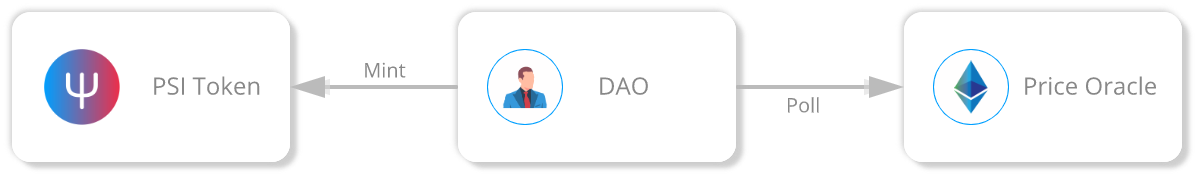
\includegraphics[scale=0.37]{diagram1}

	\end{center}

	\newpage

	\subsection{Oracle}
	The Psi protocols initial oracle is built on top of the \texttt{PSI:USDC} Uniswap v2 pair, ensuring flash loan resistant price data. New average weighted prices are polled and computed each epoch 				advancement when a \texttt{poll()} transaction is sent to the Oracle contract.

	% Oracle diagram %
	\begin{center}

		
\includegraphics[scale=0.37]{diagram2}
	
	\end{center}
	
	\subsubsection{LP Incentivizaton}
	To incentivize users to provide liquidity for the \texttt{PSI:USDC} Uniswap v2 pool an LP incentivization pool will be used. A portion of \texttt{PSI} minted in a supply expansion event will be credited to 	the LP incentivization pool. \texttt{PSI} in this pool will be distributed to users who are providing liquidity to the \texttt{PSI:USDC} Uniswap v2 pool, as proof of providing liquidity, users will have to 			stake their \texttt{UNI-V2} LP tokens from the \texttt{PSI:USDC} pair.

	\subsection{Epochs}
	The Psi protocol DAO formats time into distinct periods of approximately one day, these periods are called \textit{epochs}.  The DAO does this to simplify logic concerning several things:
	
	% List of DAO logic items %
	\begin{itemize}

		\item{Governance.}
		\item{Supply regulation.}
		\item{Flash loan resistance.}

	\end{itemize}
	
	A new epoch is entered when the previous one is \textit{advanced} by a user sending an \texttt{advance()} transaction to the DAO. During an advancement operation, state transformations can be 				applied to the Psi protocol, namely:

	% List of state tranformation operations %
	\begin{itemize}

		\item{\textit{Bond} expiry.}
		\item{Supply regulation.}

	\end{itemize}

	To incentivize users to send \texttt{advance()} transactions, the DAO mints reward \texttt{PSI} tokens to the sender of the transaction if the advancement operation is successful.
	
	Epochs become available for advancement based upon the current Ethereum block timestamp.

	\newpage

	\subsection{Staking}
	The Psi protocol only contains one token: \texttt{PSI}. As mentioned previously, the \texttt{PSI} token is a stablecoin, but it is also used as a governance token. Users can deposit their \texttt{PSI} 			tokens into the DAO, which can then be \textit{staked}. DAO votes are then allocated to the user based on the amount of \texttt{PSI} they have staked. After staking their tokens, the user is 				temporarily locked from depositing or withdrawing \texttt{PSI} tokens until the next epoch. This ensures a static balance of staked \texttt{PSI} during the staked epoch, not allowing users to increase 			or decrease their share of votes, this concept underpins the DAO's security model.

	% State diagram %
	\begin{center}

		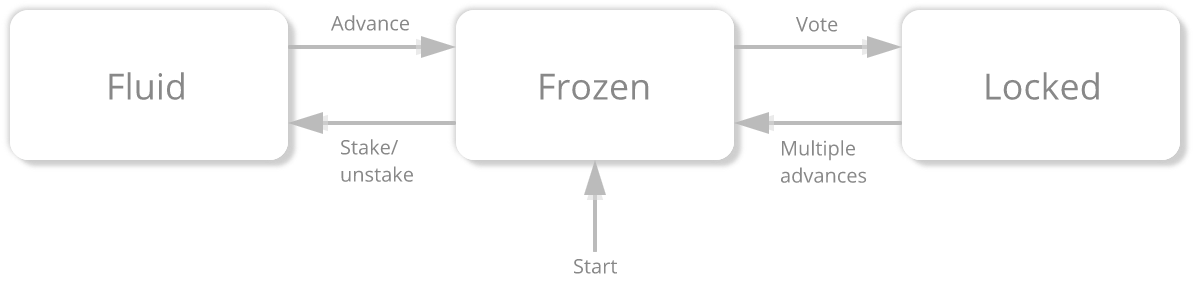
\includegraphics[scale=0.37]{diagram3}

	\end{center}

	The \texttt{Locked} state is when the DAO must lock staked \texttt{PSI} tokens for multiple epochs. This state is entered during the governance process, a will remain in that state until the 					referendum has concluded, this is to ensure that a users vote allocation does not change over the duration of the governance process.

	In short, the user can only stake and unstake when their account is in the \texttt{Frozen} or \texttt{Fluid} state, but can deposit, withdraw, vote, and receive payouts when their account is in the 				\texttt{Frozen} or \texttt{Locked} state.

	\subsection{Stability Mechanism}
	The \texttt{PSI} stablecoin utilizes an elastic supply governed by its DAO to adjust to changes in demand while targeting a fixed price. Supply can be balanced with the following equality:
	
	% Supply equality %
	\begin{center}

		$supply_n \cdot price_n = supply_{n + 1} \cdot 1.00$
	
	\end{center}

	From this, we can determine the necessary change in supply to regulate price:
	
	% Change in supply %
	\begin{center}

		$\Delta supply = supply_n \cdot (price_n - 1.00)$

	\end{center}

	To prevent \textit{debt} from overtaking supply, we instead use \textit{net supply} (\textit{supply} less \textit{debt}) in the above calculation which allows debt to approach supply asymptotically. 			\newline

 	The DAO adjusts the supply of the \texttt{PSI} token by incentivizing users to engage in supply regulating activities, notably:
	
	%List of supply regulation operations%
	\begin{itemize}
	
		\item{Supply expansion: \textit{bond} redemption.}
		\item{Supply contraction: \textit{bond} purchase.}
	
	\end{itemize}

	\newpage

	\subsubsection{Supply Expansion}
	For positive $\Delta supply$, new \texttt{PSI} tokens are minted by the DAO and distributed as follows:
	
	% Distribution %
	\begin{enumerate}

		\item{Credited to the bond redemption pool, for outstanding bonds, until pool can cover entirety of outstanding bonds.}
		\item{Immediately burned to reduce \textit{debt} until \textit{debt} reaches zero.}
		\item{Any surplus is credited proportionately to staked \texttt{PSI} holders.}

	\end{enumerate}

	\subsubsection{Supply Contraction}
	To contract the supply of the \texttt{PSI} token, users must be incentivized to burn their tokens. To do this, \textit{bonds} are offered to users, which are redeemable for a premium quantity of 				\texttt{PSI} tokens in the future.
	To contract by $\Delta supply$, the DAO issues the equivalent amount of \textit{debt}, which marks the current amount of \texttt{PSI} tokens that may be burnt in exchange for \texttt{bonds}.

	\subsection{Bond Market}
	To incentivize the exchange of \texttt{PSI} tokens for bonds, an AMM is created over the current \textit{debt ratio}. As the debt ratio increases, so does the bond premium, which ensures the correct 			incentivization even during periods of extreme down regulation.
	The debt ratio is \textit{expected} to be non-zero during periods of supply contraction as it is the mechanism for which the market prices the bond premium.
	First the \textit{debt ratio R} is defined as:

	\begin{center}

		$R = $ \Large{$\frac{debt}{supply}$}

	\end{center}

	An ideal premium curve would have \textit{zero} premium at \textit{zero} debt, with asymptotically increasing premium as debt approaches supply. With this in mind, we can define our premium 			curve over R as:
	
	\begin{center}

		$premium(R) = $ \Large{$\frac{1}{3(1 - R)^2} - \frac{1}{3}$}

	\end{center}

	\begin{center}

		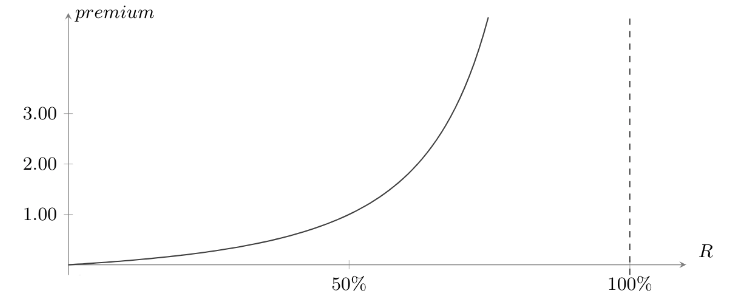
\includegraphics[scale=0.6]{graph1}

	\end{center}

	\newpage

	\subsubsection{Calculating bond amount}
	With our \textit{premium} curve defined, we can now calculate how an order of size \textit{n} will be priced. We begin by defining \textit{R'}, the resulting debt ratio after execution as,
	\begin{center}
		\begin{equation}
		\label{eq1}
			\begin{split}
				premium & = \frac{\int_{R'}^{R} premium(R)\, dR}{R - R'}\\
				& = \frac{1}{3(1 - R)(1 - R')} - \frac{1}{3}
			\end{split}
		\end{equation}
	\end{center}
	
	\begin{center}
		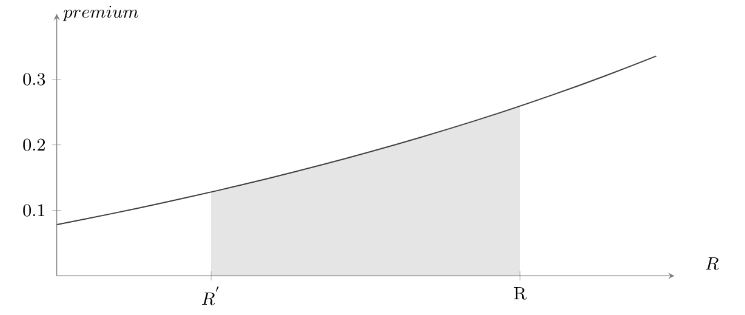
\includegraphics[scale=0.55]{graph2}
	\end{center}
	
	Once the premium is determined, we can then calculate the resulting bond amount for the order.
	
	\begin{center}
		$bonds = n \cdot (1 + premium)$
	\end{center}

	\subsubsection{Bond Redemption}
	Bonds entitle holders to a 1:1 redemption of \texttt{PSI} tokens at some time in the future. When there is a supply expansion event, newly minted \texttt{PSI} tokens are first credited to the 					redeemable pool. This pool is first-come first-served for any current bond holder.
	This ensures that a queue does not form, disincentivizing new bond purchasers, as debt increases. Further, bonds are valid for 90 days, after which they will expire and no longer be redeemable. These 	are key to mitigating downward spiral events prevalent in similar stability mechanism designs.

	\subsection{Governance}
	The DAO is fully self governing at launch. A new DAO implementation may be proposed at any time by any curretn stakeholder with at least 1\% of the current DAO stake.
	Voters have 7 days to choose to either \texttt{approve} or \texttt{reject} the candidate implementation. If a quorum of 33\% is reached, and more votes approve, then the new implementation may 			be committed.

	By only allowing full implementation upgrades, even for simple constant modifications, we ensure a lightweight governance process.


\end{document}
